%%----------------------------------------------------------------------------
%% Presentatie HoGent Bedrijf en Organisatie
%%----------------------------------------------------------------------------
%% Auteur: Bert Van Vreckem [bert.vanvreckem@hogent.be]

\documentclass{beamer}

%==============================================================================
% Aanloop
%==============================================================================

%---------- Packages ----------------------------------------------------------

\usepackage{graphicx,multicol}
\usepackage{comment,enumerate,hyperref}
\usepackage{amsmath,amsfonts,amssymb}
\usepackage{tikz}
\usepackage[dutch]{babel}
\usepackage[utf8]{inputenc}
\usepackage{multirow}
\usepackage{eurosym}
\usepackage{listings}
\usepackage[T1]{fontenc}
\usepackage{lmodern}
\usepackage{textcomp}
\usepackage{framed}
\usepackage{wrapfig}

%---------- Configuratie ------------------------------------------------------

\usetikzlibrary{arrows,shapes,backgrounds,positioning,shadows}

\usetheme{hogent}

%---------- Commando-definities -----------------------------------------------

\newcommand{\tabitem}{~~\llap{\textbullet}~~}

%---------- Info over de presentatie ------------------------------------------

\title[Intro]{Coding For Dummies}
\author{Jens {Buysse}}
\date{\today}

%==============================================================================
% Inhoud presentatie
%==============================================================================

\begin{document}

%---------- Front matter ------------------------------------------------------

% Dia met het HoGent logo
\HoGentLogo

% Titeldia met faculteitslogo
\titleframe

%---------- Inhoud ------------------------------------------------------------

\begin{frame}
  \frametitle{Inhoud}

  \tableofcontents
\end{frame}


\section{De eerste codes}
\sectionframe{When Cryptography is outlawed, bayl bhgynjf jvyy unir cevinpl \\\begin{flushright}
		-- John Perry Barlow
\end{flushright} }
\begin{frame}{Cryptografie}
	Het woord \textcolor{HoGentBlue}{cryptografie} betekent letterlijk  \textcolor{HoGentBlue}{‘geheim schrijven’} of  \textcolor{HoGentBlue}{‘verborgen schrijven’}, het is voortgekomen uit de 2 griekse woorden 
	\begin{itemize}
		\item kruptos en
		\item graphein
	\end{itemize}
	 wat samen ‘geheim schrijven’ betekent.
\end{frame}

\begin{frame}{De eerste codes}
	Zowel de Romeinen als de Grieken verdiepten zich in de grondbeginselen van cryptografie. 
	
	\begin{itemize}
		\item Optische signalen m.b.h.v. toortsen
		\item vlaggen
		\item spiegels
		\item \dots
	\end{itemize}
\end{frame}

\begin{frame}{De eerste codes}
	\begin{figure}
		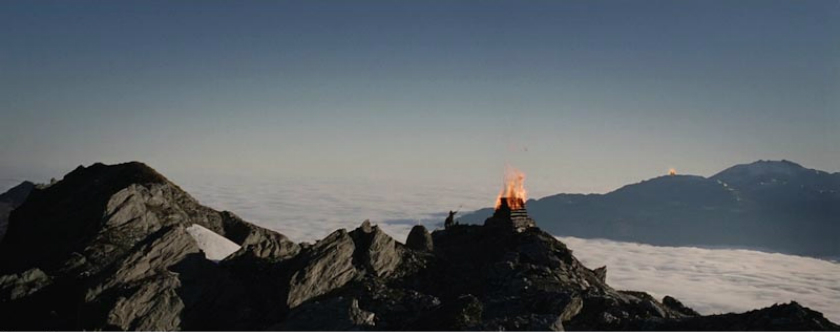
\includegraphics[width=\textwidth]{img/toorts.jpg}
	\end{figure}
\end{frame}

\begin{frame}{Polybius}
	Code ontwikkeld door Griekse militair.
	\[ \begin{bmatrix}
		& 1  & 2  & 3  & 4 & 5\\ 
		1 & A  & B  &  C & D & E\\ 
		2 & F & G  & H  & I  & J \\ 
		3 & K & L  & M  & N  & O \\ 
		4 & P & Q & R & S  &  T\\ 
		5 & V & W & X & Y & Z  
	\end{bmatrix}  \]
	Wat betekent volgend geheimschrift?
	\[ \begin{bmatrix}
12 & 53 & 34 & 54 & 15 & 43 & 51 & 12 & 11 & 15 \\ 
53 & 34 & 44 & 54 & 32 & 51 & 21 & 53 &23 &41 
\end{bmatrix} \]
\end{frame}

\begin{frame}{Polybius}
	Er werden twee reeksen van fakkels opgesteld:
	\begin{enumerate}
		\item Eerste 5 fakkels duiden de rij aan
		\item Tweede 5 fakkels duiden de kolom aan
	\end{enumerate}
\end{frame}

\begin{frame}{Aenas' Telegraaf}
		\begin{figure}
		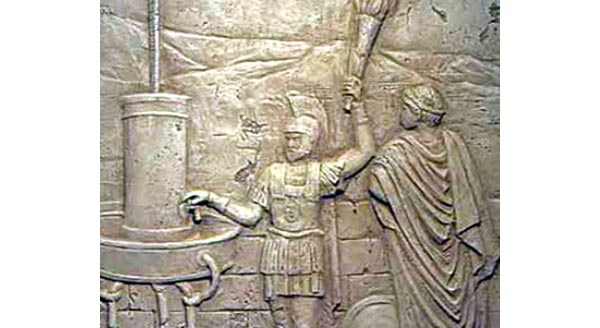
\includegraphics[width=\textwidth]{img/aenas.jpg}
	\end{figure}
\end{frame}

\begin{frame}{Aenas' Telegraaf}
	\begin{enumerate}
		\item Partij A heft een brandende fakkel
		\item Partij B heft ten antwoord ook een brandende fakkel
		\item Partij A laat fakkel zaken en kranen worden open gezet
		\item Partij A heft opnieuw brandende fakkel op zodat kranen gesloten kunnen worden.
	\end{enumerate}
\end{frame}

\begin{frame}[fragile]{Caesarscode}
	Elke letter wordt vervangen door de letter die een afgesproken aantal plaatsen (bv. 3) verder in het alfabet staat. 
	

	\begin{block}{Code}
	EDG LV D SODQ ZKLFK FDQQRW EHDU D FKDQJH
	\end{block}

\end{frame}

\begin{frame}[fragile]{Caesarscode - zwaktes}
	Wat zijn de zwaktes van deze codering en hoe zou je deze aanpakken?
	\pause
	\begin{itemize}
		\item Biedt slechts 25 mogelijkheden tot versleuteling. (Computer kan dit makkelijk kraken)
		\item De letter E komt heel erg vaak voor in de taal. Door te tellen welke letter het meest voorkomt kan je al goed raden wat de E zal zijn. 
		\item Je weet ook al wat de woorden zijn.
	\end{itemize}

\begin{center}
	\begin{block}{Code}
ROHXD VDBCK ANJTC QNUJF MXRCC XBNRI
NYXFN ARWJU UXCQN ALJBN BXKBN AENRC
\end{block}
\end{center}
\end{frame}

\begin{frame}[fragile]{Scytale}
	\begin{figure}
		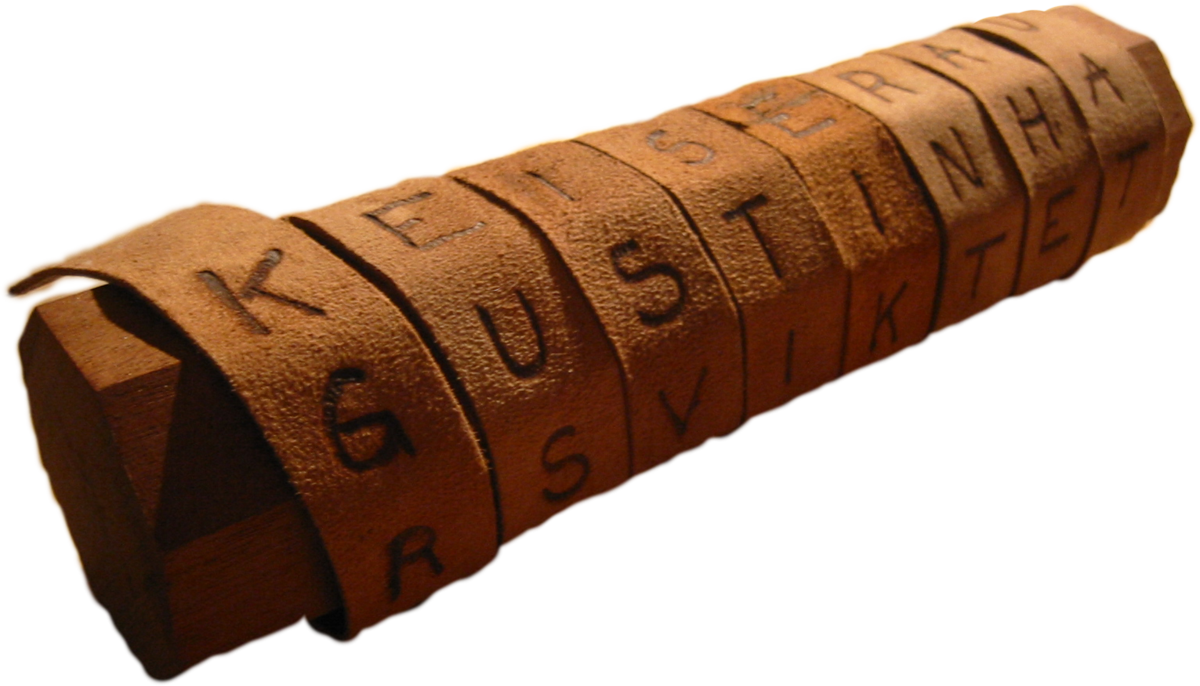
\includegraphics[width=\textwidth]{img/scytale}
	\end{figure}

\begin{block}{Code}
	ANACD DEIOR SUTWB AOTIR FNSUE ELNTF EHRMA IYNE
\end{block}

\end{frame}

\section{Iets formeler}
\sectionframe{Cryptography shifts the balance of power from those with a monopoly on violence to those who comprehend mathematics and security design. \\\begin{flushright}
		Jacob Appelbaum
\end{flushright}}

\begin{frame}{Adam, Alice \& Eve}
	\begin{figure}
		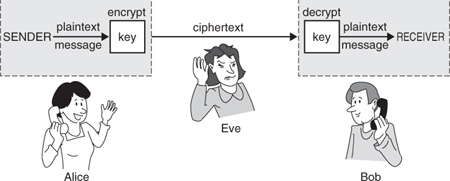
\includegraphics[width=\textwidth]{img/adameve.jpg}
	\end{figure}
\end{frame}

\begin{frame}{Cryptografieindeling}
	\begin{description}
		\item[Symmetrisch] Wanneer de sleutel om te versleutelen en ontsleutelen dezelfde is. Versleuteling kan enkel veilig gebeuren wanneer er een veilige sleuteluitwisseling tussen Alice en Bob gebeurd is.
	\item[Assymetrisch] Of ook publieke sleutel cryptografie waarbij het versleutelen en ontsleutelen met een verschillende sleutel moet. 
\end{description}
We merken op dat hedendaagse versleutelingsmechanismen vaak een gelaagde combinatie van bovengenoemde types zijn.
\end{frame}

\begin{frame}{Enkele definities}
	\begin{description}
		\item[Plaintext / Cleartext] Het ongecodeerde bericht. 
			
		\item[Encryption] de codering van de plaintext
		\item[Ciphertext] 
		
		Dit is de uiteindelijke tekst, in versleutelde vorm. Bij een goed gecodeerde tekst is de ciphertext een onbegrijpelijke boodschap, waaruit onbevoegden praktisch onmogelijk de plaintext kunnen halen.
		\item[Decryption] 
		
		De decryption is de stap die de ontvanger uitvoert om het originele bericht weer uit de ciphertext te halen. 
		\item[Key] 
		
		De key is   de sleutel die je nodig hebt om een ciphertext te decoderen. 
		\item[Cryptanalysis] 
		
		Dit begrip houdt het kraken van een gecodeerde tekst in. 
		\item[Cryptology] 
		
		Cryptologie is een net iets minder ruim begrip dan Cryptografie. Bij cryptologie wordt namelijk alleen de wiskundige kant van de cryptografie bestudeerd.
	\end{description}

\end{frame}

\begin{frame}{Kraakpogingen - Kerckhoffs' principes}
	
	\begin{enumerate}
		\item Het systeem dient, zelfs als het in theorie niet onbreekbaar is, in de praktijk onbreekbaar te zijn. \pause
		\item \textcolor{HoGentAccent1}{Het ontwerp van het systeem behoort niet geheim te hoeven zijn en dient, indien gecompromitteerd, de correspondenten niet te kunnen schaden.}\pause
		\item De sleutel moet onthoudbaar zijn zonder notities en dient makkelijk veranderd te kunnen worden.\pause
		\item De cryptogrammen moeten overgebracht kunnen worden door middel van telegrafie.\pause
		\item Het apparaat of de documenten dienen draagbaar te zijn en te kunnen worden bediend door een enkel persoon.\pause
		\item Het systeem dient gemakkelijk te zijn, niet onderhevig aan kennis van allerlei regels of aan mentale inspanning\pause
\end{enumerate}
	\textcolor{HoGentAccent1}{Belangrijk: \textit{principe van Kerckhoffs}}: de veiligheid van een cryptografisch systeem mag niet van de geheimhouding van het versleutelingssysteem maar slechts van de geheimhouding van de sleutel afhangen.

\end{frame}

\begin{frame}{Kraakpoging - Brute Force}
	\brightbox{Brute force (Engels voor "brute kracht") is het gebruik van rekenkracht om een probleem op te lossen met een computer zonder gebruik te maken van algoritmen of heuristieken}

\begin{itemize}
	\item 	 De methode bestaat uit het botweg uitproberen van alle mogelijke opties, net zo lang tot er een gevonden is die overeenkomt met de gewenste invoer.
\end{itemize}
	
\end{frame}

\begin{frame}{Combo Attack}
	Gebruik een woordenboek en plak de verschillende woorden tezamen.
	\begin{itemize}
		\item dictionary1.txt \& dictionary2.txt
		\item pass $ \rightarrow $ password, passpass, passlion
		\item word $ \rightarrow $ wordpass, wordword, wordlion
		\item lion $ \rightarrow $ lionpass, lionword, lionlion 
	\end{itemize}
\end{frame}

\begin{frame}{Combo Attack}
Combo attack, maar met de mogelijkheid een willekeurige reeks letters toe te voegen
	\begin{itemize}
	\item dictionary.txt \& abcde
	\item pass $ \rightarrow $ passAbc, passBcd, passCde
	\item word $ \rightarrow $ wordAbc, wordBcd, wordCde
	\item lion $ \rightarrow $ lionAbc, lionBcd, lionCde
	\end{itemize}
\end{frame}

\begin{frame}{Use Case: Wordpress websites}
	Als je gebruikt maakt van Wordpress ben je kwetsbaar voor Brute Force attacks.
	
	Je kan hiertegen een aantal eenvoudige maatregelen gebruiken:
	\begin{enumerate}
		\item Sterke paswoorden gebruiken
		\item De admingebruikersnaam veranderen
		\item Het aantal loginpogingen beperken
		\item Loginpagina anders noemen
		\item IP adressen die toegang hebben beperken
		\item CAPTCHA toevoegen
	\end{enumerate}
\end{frame}

\section{RSA}
\sectionframe{\begin{center}
		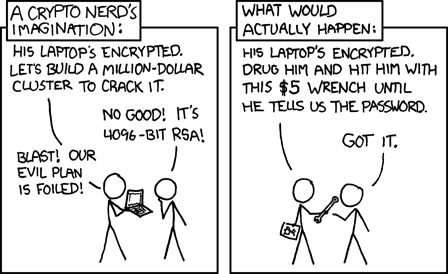
\includegraphics[width=\textwidth]{img/security.png}
\end{center}}


\begin{frame}{RSA}

\textbf{-----BEGIN PUBLIC KEY-----}\\
MIIBIjANBgkqhkiG9w0BAQEFAAOCAQ8AMIIBCgKCAQEAvUWEGue
PMihBxG8/mhi1z9YdCXEDk01iqLcYEKa4uPfPao0DAU2/4hSkWu
JCgBkAzJns8hz7DKskdRrTnhG1rcomyLFz07GFq1qkmpc6bL1UW
UNsdIOtu0CsgbtdeFW5OMJhezljf/jvuYRpE+eNPwHmg0233JvN
TVQ2ZNUO9eXX7gt1qYKZiHR3warYYE+7ro6BOwY3pBOG8iIm3zj
u2ioICGFH/hd9Jd19+mZwWneccYv89W1eSyPYg5yBWIIYLSFZA9
imlO0Xe3/ifRQyDjaE5YbTQt6/CkBYmObp009Exp3QwPnpYLTKM
zhjfgk+5Bg3O2wVVX+1ny7QqLSHrQIDAQAB\\
\textbf{-----END PUBLIC KEY-----}
\end{frame}

\begin{frame}{RSA}
	
\includegraphics[width=\textwidth]{img/secret.png}
\end{frame}

\begin{frame}{RSA}
	
\includegraphics[width=\textwidth]{img/bank.jpg}
\end{frame}

\begin{frame}{RSA}
	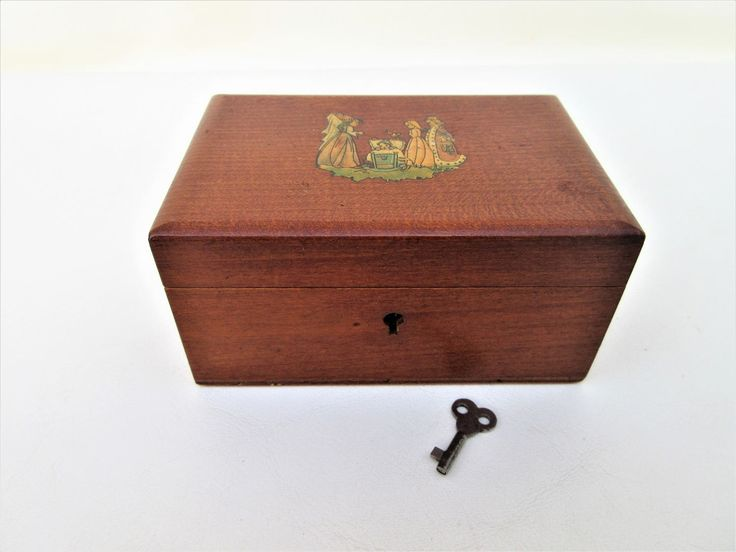
\includegraphics[width=\textwidth]{img/box.jpg}
\end{frame}

\begin{frame}{RSA}
	\begin{columns}
		\begin{column}[T]{0.5\textwidth}
			
\includegraphics[width=\textwidth]{img/bank.jpg}
		\end{column}
	
		\begin{column}[T]{0.5\textwidth}
			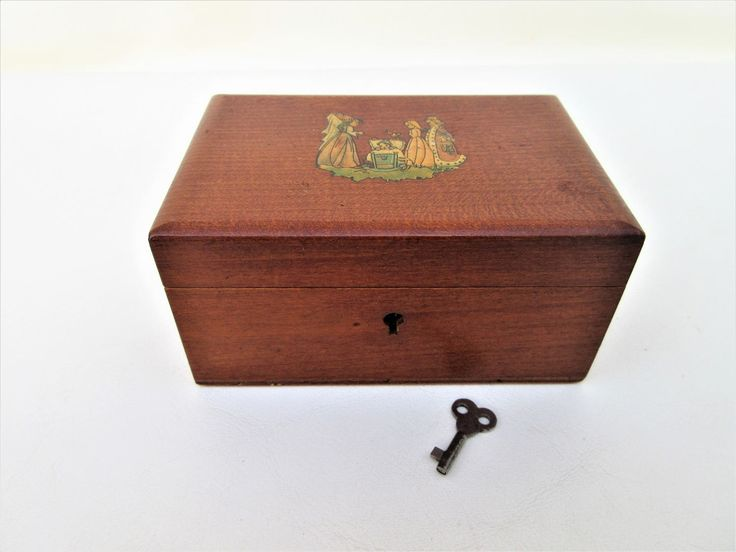
\includegraphics[width=0.3\textwidth]{img/box.jpg}
			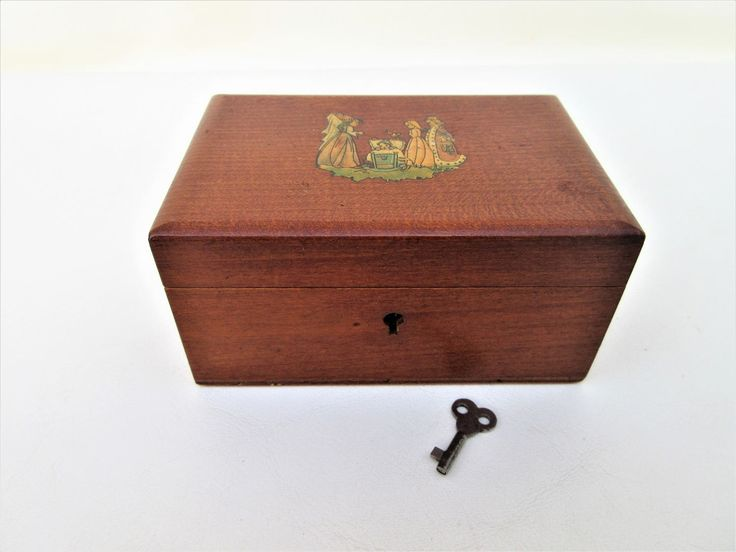
\includegraphics[width=0.3\textwidth]{img/box.jpg}
			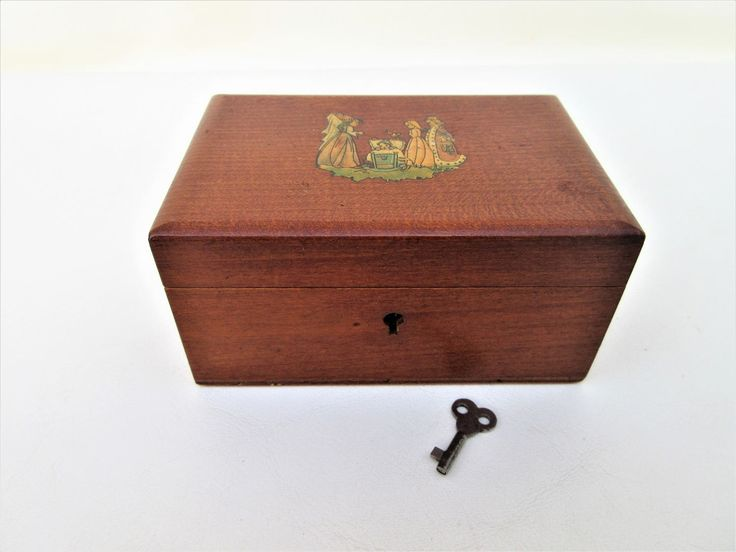
\includegraphics[width=0.3\textwidth]{img/box.jpg} \\
						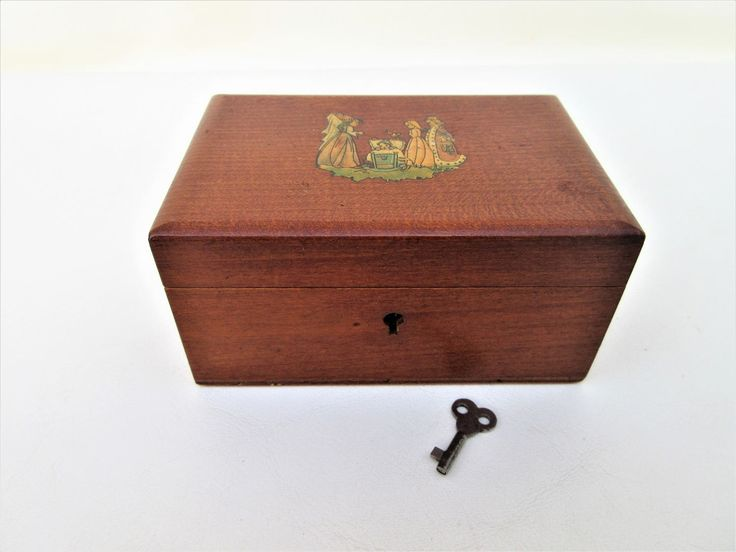
\includegraphics[width=0.3\textwidth]{img/box.jpg}
			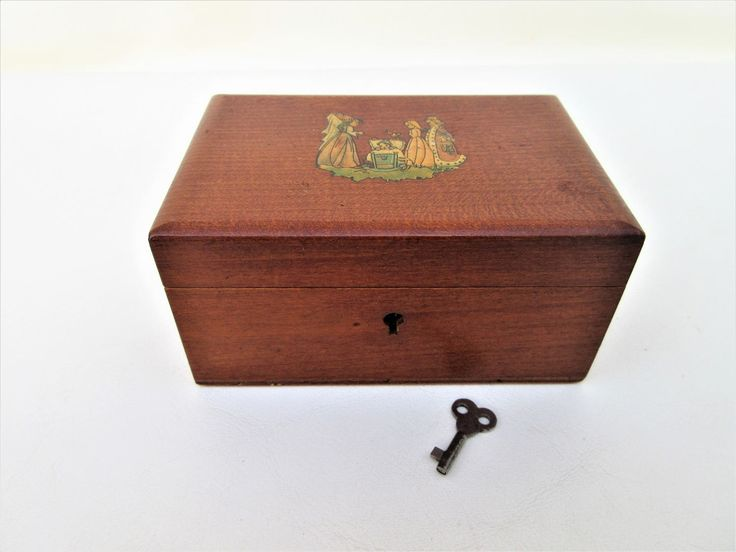
\includegraphics[width=0.3\textwidth]{img/box.jpg}
			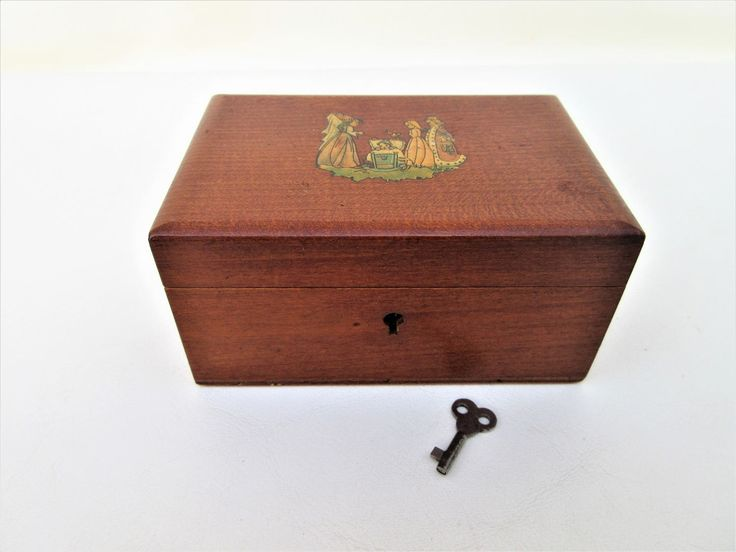
\includegraphics[width=0.3\textwidth]{img/box.jpg} \\
						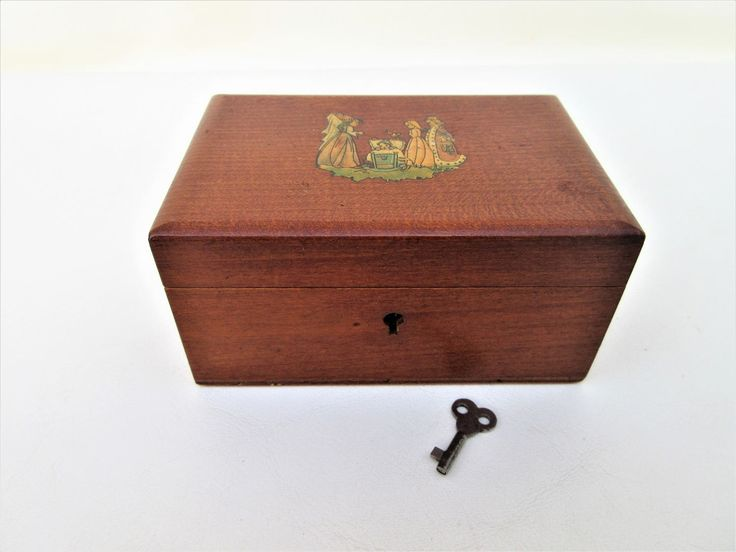
\includegraphics[width=0.3\textwidth]{img/box.jpg}
			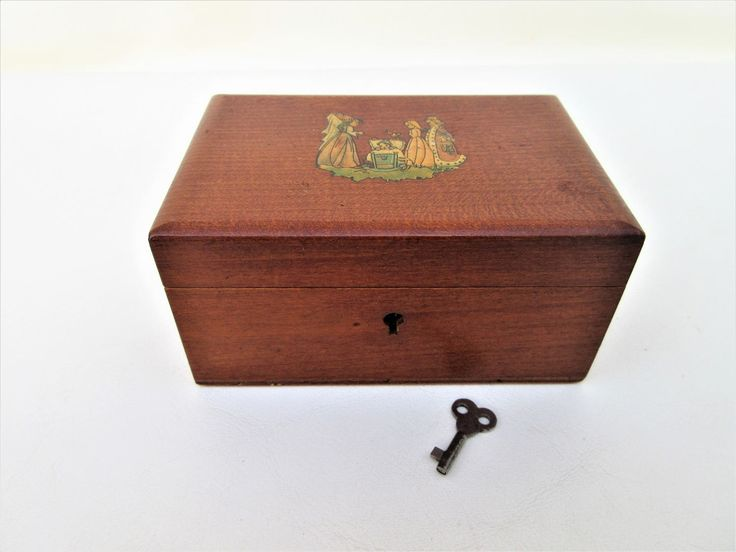
\includegraphics[width=0.3\textwidth]{img/box.jpg}
			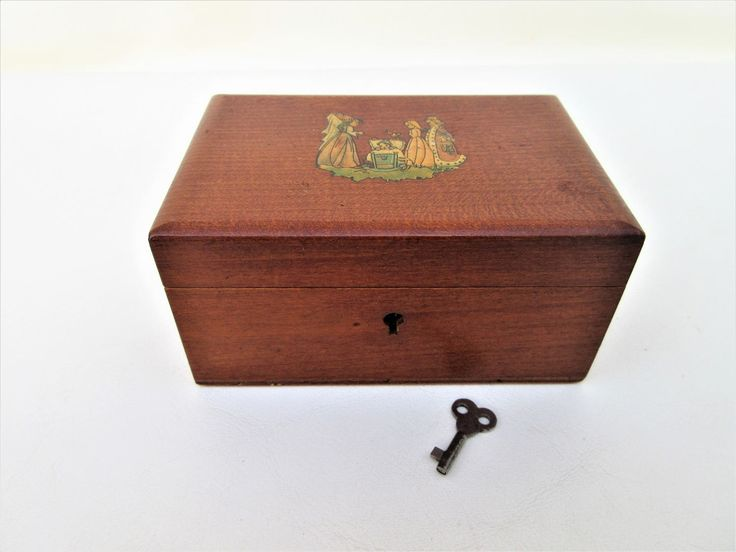
\includegraphics[width=0.3\textwidth]{img/box.jpg}
		\end{column}
	\end{columns}
\end{frame}

\begin{frame}{RSA}
	\begin{center}
		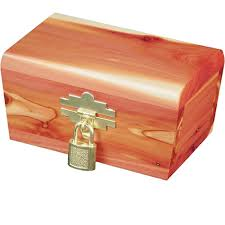
\includegraphics[width=0.4\textwidth]{img/padlock.jpeg}
	\end{center}
\end{frame}

\begin{frame}{RSA}
	\begin{columns}
		\begin{column}[T]{0.5\textwidth}
			
\includegraphics[width=\textwidth]{img/bank.jpg}
		\end{column}
		
		\begin{column}[T]{0.5\textwidth}
			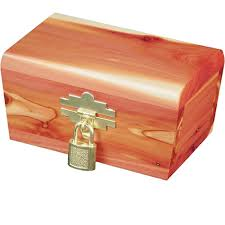
\includegraphics[width=0.3\textwidth]{img/padlock.jpeg}
			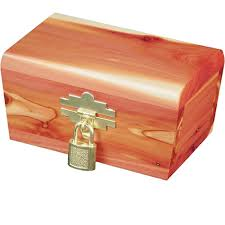
\includegraphics[width=0.3\textwidth]{img/padlock.jpeg}
			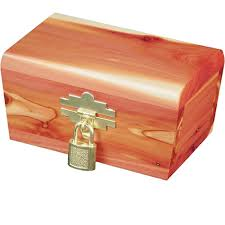
\includegraphics[width=0.3\textwidth]{img/padlock.jpeg} \\
			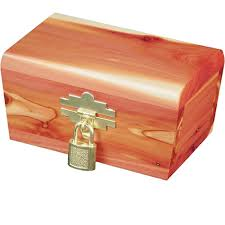
\includegraphics[width=0.3\textwidth]{img/padlock.jpeg}
			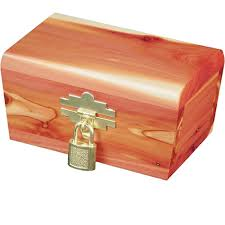
\includegraphics[width=0.3\textwidth]{img/padlock.jpeg}
			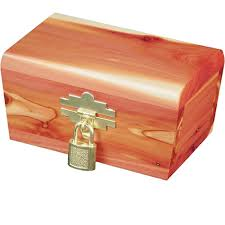
\includegraphics[width=0.3\textwidth]{img/padlock.jpeg} \\
			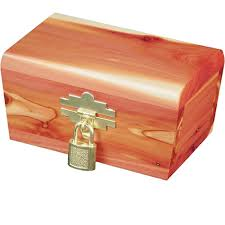
\includegraphics[width=0.3\textwidth]{img/padlock.jpeg}
			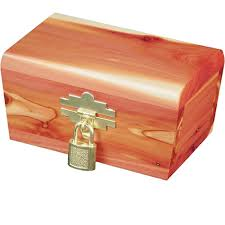
\includegraphics[width=0.3\textwidth]{img/padlock.jpeg}
			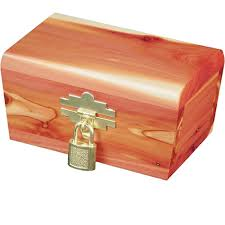
\includegraphics[width=0.3\textwidth]{img/padlock.jpeg}
		\end{column}
	\end{columns}
\end{frame}

\subsection{Modulo rekenen}


\begin{frame}{Modulo rekenen}
	\begin{columns}
		\begin{column}[T]{0.5\textwidth}
			Stel dat het op een moment 20 uur is  , en je telt daar 7 uur bij op. Dan zou het volgens gewone rekenmethodes dus 20 + 7 = 27 uur moeten zijn.
			
			Maar niemand noemt dat 27 uur, iedereen zegt 3 uur. Dat komt natuurlijk omdat het de volgende dag is geworden en die 24 uur van de vorige dag interesseren ons niet zoveel meer.
		\end{column}
		
		\begin{column}[T]{0.5\textwidth}
				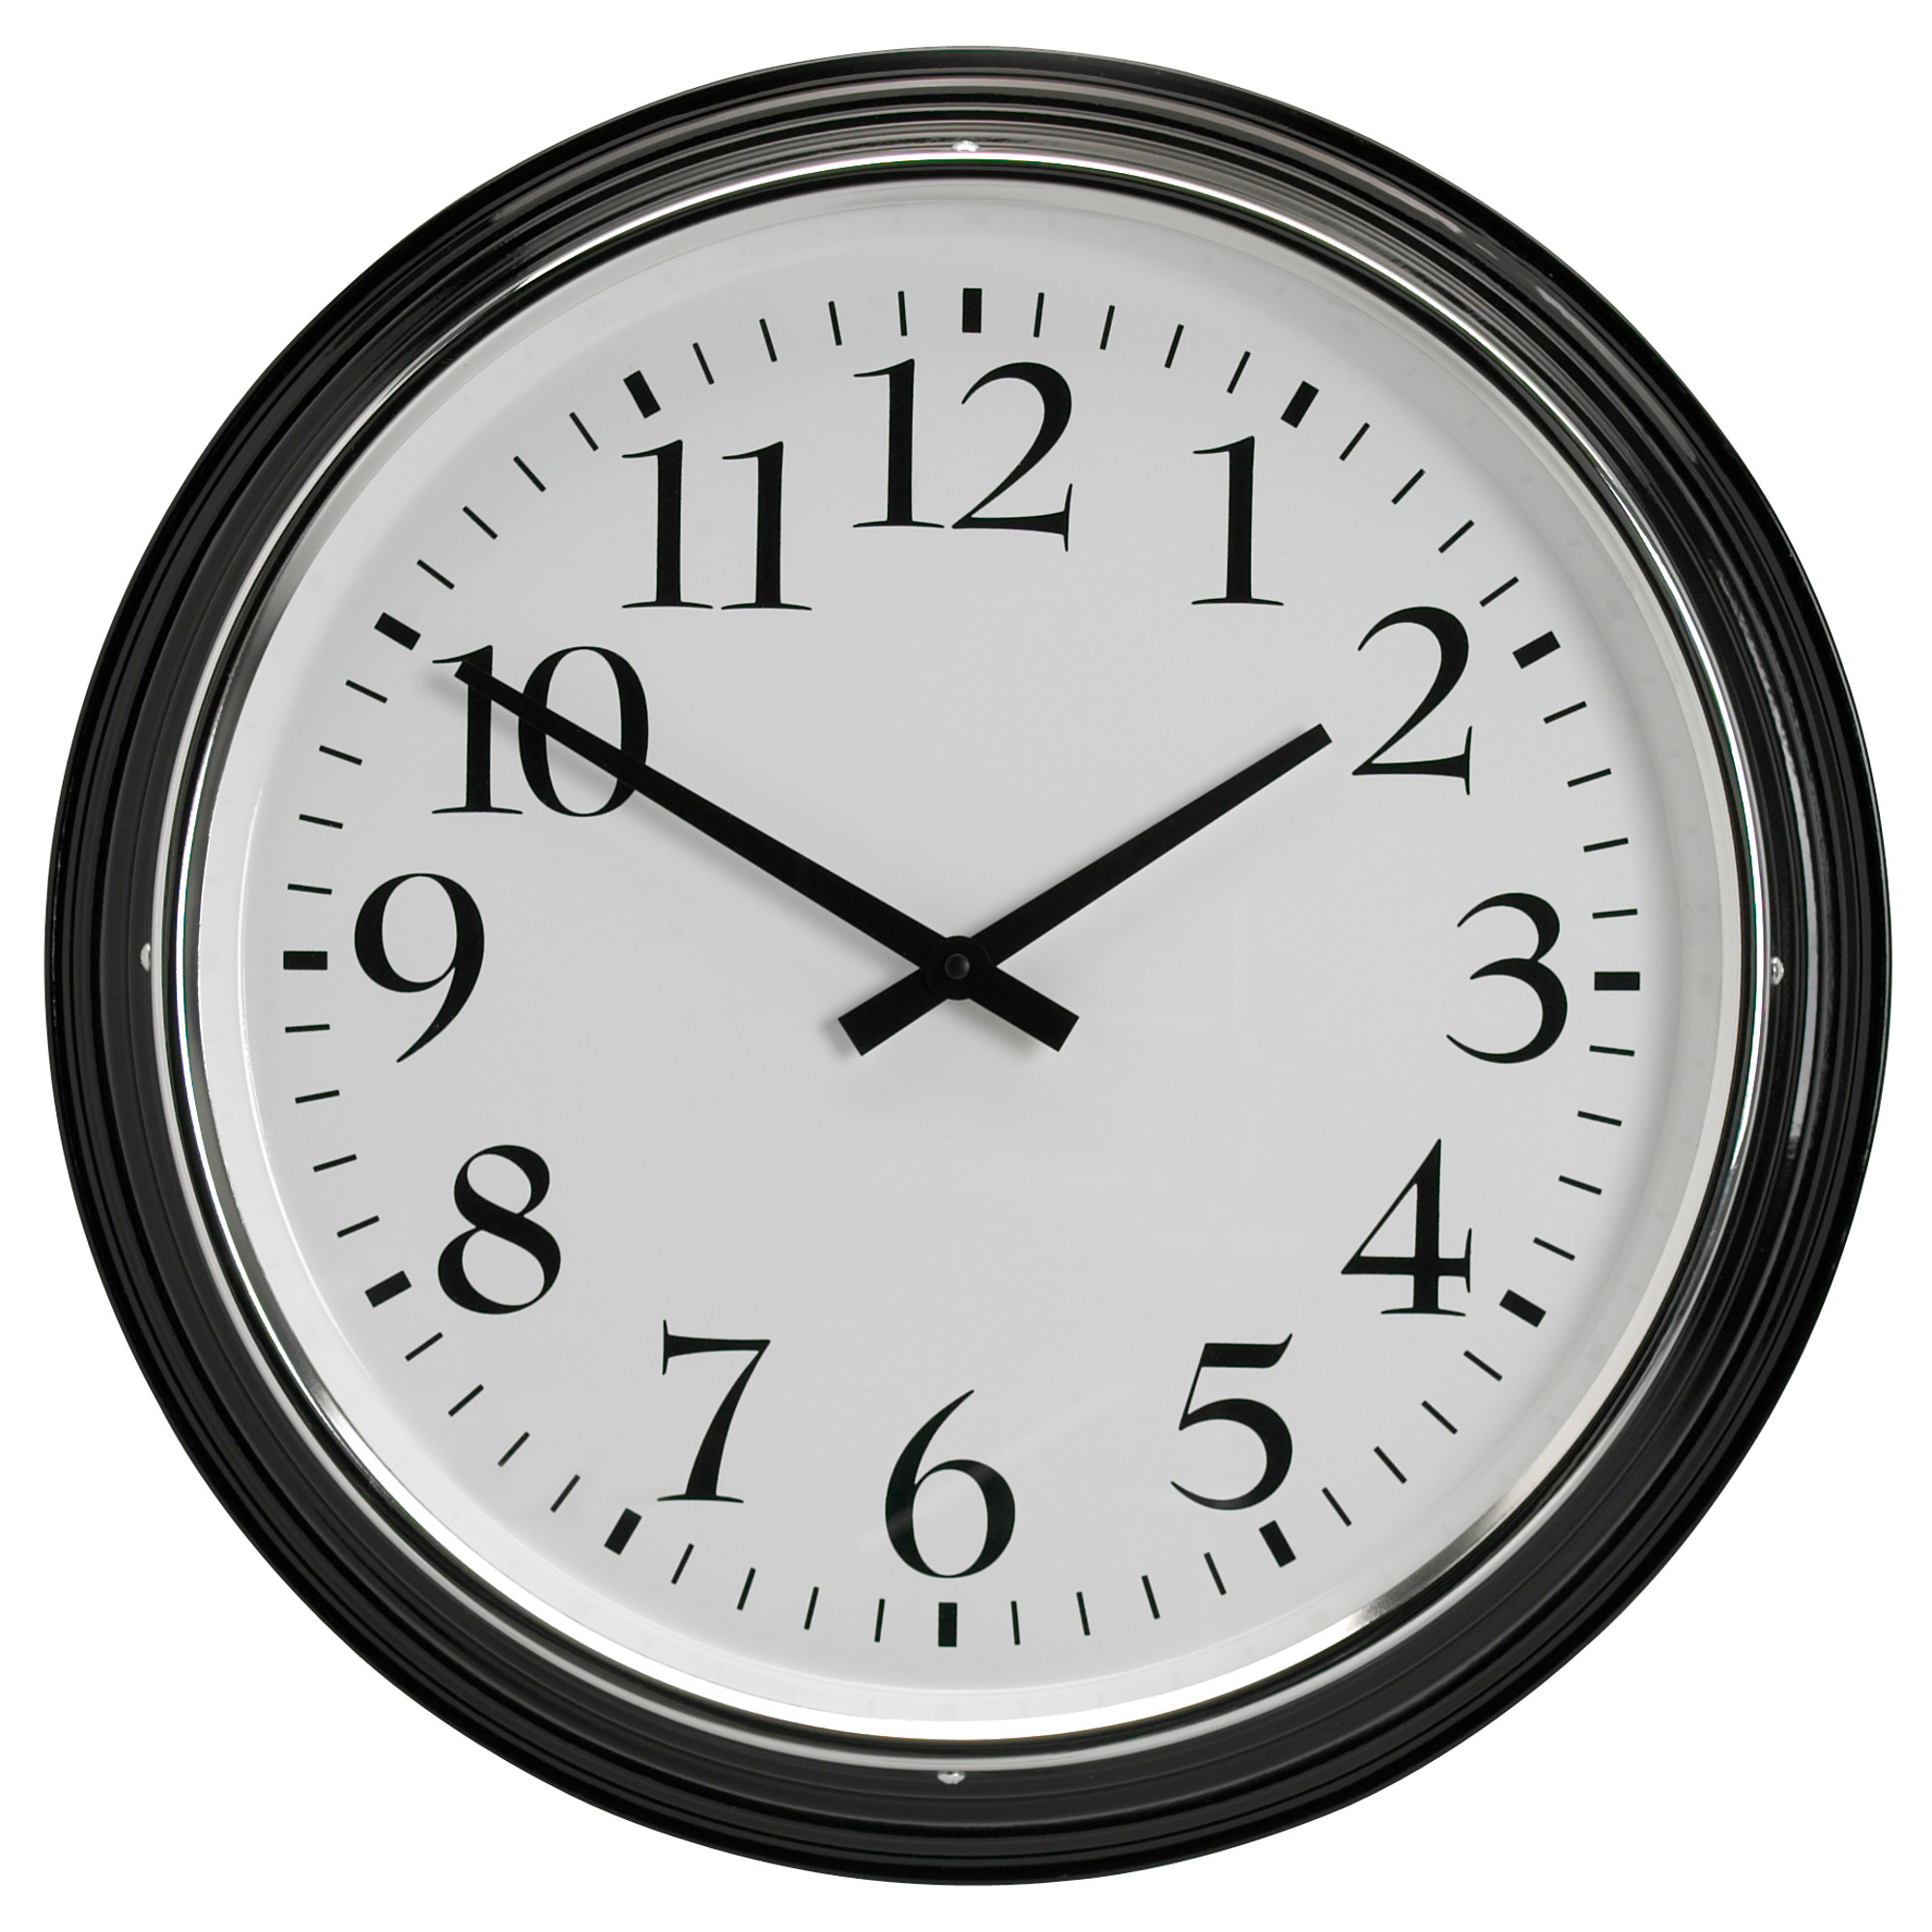
\includegraphics[width=\textwidth]{img/clock.jpg}
		\end{column}
	\end{columns}
\end{frame}

\begin{frame}{Modulo rekenen}

	Zij $n$ n een natuurlijk getal ongelijk $\neq 0$, dan heten de twee gehele getallen $a$ en $b$ congruent modulo $n$, genoteerd:
	
	\[ 
		a \equiv b \pmod{n}
	\]
	
	als hun verschil $a - b$ een geheel veelvoud is van $n$.
	
	Het getal $n$ wordt de modulus genoemd.
	
\end{frame}

\begin{frame}{Voorbeelden modulo rekenen}
	\begin{eqnarray}
			26  \pmod{8} &= \pause 2 \\
			-13 \pmod{8} &= \pause 3 \\
			257 \pmod{8} &= \pause 1 
	\end{eqnarray}
\end{frame}

\begin{frame}{Andere notatie}
	\begin{eqnarray}
	26  \pmod{8} &=  2 + k \times 8 \\
	-13 \pmod{8} &= 3 + k \times 8\\
	257 \pmod{8} &=  1 + k \times 8
	\end{eqnarray}
\end{frame}

\begin{frame}{Modulo Rekenregels$_1$}
	\[ a \pmod{m} + b \pmod{m}  =  (a + b)  \pmod{m}\]
\end{frame}

\begin{frame}{Modulo Rekenregels$_2$}
	\[ a \pmod{m} \times b \pmod{m}  =  (a \times b)  \pmod{m}\]
\end{frame}

\begin{frame}{Modulo Rekenregels$_3$}
	\[ (a \pmod{m})^n  =  a^n  \pmod{m}\]
\end{frame}

\begin{frame}{Toepassing bankrekeningen - Nederland}
	\[ c_1c_2c_3c_4c_5c_6c_7c_8c_9\]
	Nu is $c_9$ zo gekozen dat, als je dit getal  $\pmod{11}$ neemt, er 0 uitkomt.
	
\end{frame}

\begin{frame}{Toepassing bankrekeningen - Nederland}
	\[ 45824365c_9\]
	bepaal
	\[ 9 \times 4 + 8 \times 5 + \dots + 2 \times 5 \]
	Kies $c_9$ zodat $\sum_i^9  i \times c_i \pmod{11} = 0$ \\
	Als de som 204 is dan moet $c_9 = 5$ 
	
\end{frame}

\sectionframe

\begin{frame}{Omgekeerde functie}
	Men verstaat onder de inverse van een variabele $x$ ten opzichte van een bepaalde binaire bewerking het getal $x^{-1}$, waarvoor het resultaat van de bewerking toegepast op $x$ en de inverse het neutrale element van die bewerking oplevert.
	
	\[
		7 \times 328 = 2296
	\]
	Dit is eigenlijk een versleuteling van 7.
	
	\[ 
		2296 * \times \frac{1}{328} = 7
	\]
	
	of 
	\[ 
		328 \times \frac{1}{328} = 1
	\]
\end{frame}

\begin{frame}{RSA Algoritme : stap 1}
	\begin{columns}
		\begin{column}[T]{0.5\textwidth}
			Neem 2 grote priemgetallen (100 cijfers of meer). 
			Laten we die getallen $p_1$ en $p_2$ noemen.
		\end{column}
			\begin{column}[T]{0.5\textwidth}
				Voorbeeld
		\[ p_1 = 5 \wedge  p_2 = 7\]
		\end{column}
	\end{columns}
	
	

\end{frame}

\begin{frame}{RSA Algoritme : stap 2}
	\begin{columns}
		\begin{column}[T]{0.5\textwidth}
Vermenigvuldig $p_1$ en $p_2$. 

\[ m = p_1 \times p_2  \]
Dit noemen we de modulus en vormt een deel van de publieke sleutel. 
		\end{column}
		\begin{column}[T]{0.5\textwidth}
			Voorbeeld
			\[ p_1 = 5 \wedge  p_2 = 7\]
			\[ 7 \times 5 = 35 = m \]
		\end{column}
	\end{columns}	
\end{frame}

\begin{frame}{RSA Algoritme : stap 3}
	\begin{columns}
		\begin{column}[T]{0.5\textwidth}
			Bereken een getal $\Phi$ =  het aantal getallen kleiner dan $m$ dat geen priemfactor met $m$ gemeenschappelijk heeft
		\end{column}
		\begin{column}[T]{0.5\textwidth}
			Voorbeeld

		\end{column}
	\end{columns}	
\end{frame}

\begin{frame}{Priemfactoren?}
	Priemgetallen zijn de bouwstenen van alle andere getallen:  elk getal kan opgedeeld worden in priemfactoren. 
	
	Bv. 
	\[
		12 = 4 \times 3 = 2 \times 2 \times 3 = 2^2 \times 3
	\]
	
	
\end{frame}

\begin{frame}{RSA Algoritme : stap 3}
	\begin{columns}
		\begin{column}[T]{0.5\textwidth}
			Bereken een getal $\Phi$ =  het aantal getallen kleiner dan $m$ dat geen priemfactor met $m$ gemeenschappelijk heeft
		\end{column}
		\begin{column}[T]{0.5\textwidth}
			Voorbeeld
			\[ p_1 = 5 \wedge  p_2 = 7\]
			\[ 7 \times 5 = 35 = m \]
			$m$ is opgebouwd uit de priemfactoren 5 en 7. Dus alle getallen onder de 35 waar een 5 of een 7 inzit vallen af.  Dat zijn 5, 10, 15, 20, 25, 30, 35, 7, 14, 21, 28  dus dat zijn er 11. Dus blijven er 35 - 11 = 24 getallen over, dus Φ(35) = 24.
		\end{column}
	\end{columns}	
\end{frame}

\begin{frame}{RSA Algoritme : stap 3}
	\begin{columns}
		\begin{column}[T]{0.5\textwidth}
			Bereken een getal $\Phi$ =  het aantal getallen kleiner dan $m$ dat geen priemfactor met $m$ gemeenschappelijk heeft
		\end{column}
		\begin{column}[T]{0.5\textwidth}
			Voorbeeld
			\[ p_1 = 5 \wedge  p_2 = 7\]
			\[ 7 \times 5 = 35 = m \]
			\[ \Phi = \Phi(p_1 . p_2) = (p_1 -1) \times (p_2 -1) \]
		\end{column}
	\end{columns}	
\end{frame}

\begin{frame}{RSA Algoritme : stap 3}
	\begin{itemize}
		\item Alle getallen uit de tafel van $p_1$  vallen af, dat zijn er $p_2$
		\item Alle getallen uit de tafel van $p_2$ vallen af, dat zijn er $p_1$
		\item Maar nu hebben we het getal $p_1 \times p_2$  dubbel meegeteld, dus er moet weer eentje bij.
	\end{itemize}
	
	Dan blijft over  
	\[ ()p_1 \times p_2) - p_1 - p_2 + 1  =   (p_1 - 1)\times(p_2 - 1) \]
\end{frame}

\begin{frame}{RSA Algoritme : stap 3}
	\begin{columns}
		\begin{column}[T]{0.5\textwidth}
			Bereken een getal $\Phi$ =  het aantal getallen kleiner dan $m$ dat geen priemfactor met $m$ gemeenschappelijk heeft
		\end{column}
		\begin{column}[T]{0.5\textwidth}
			Voorbeeld
			\[ p_1 = 5 \wedge  p_2 = 7\]
			\[ 7 \times 5 = 35 = m \]
			\[ \Phi(35) =4 \times 6 = 24 \]
		\end{column}
	\end{columns}	
\end{frame}

\begin{frame}{RSA Algoritme : stap 4}
	\begin{columns}
		\begin{column}[T]{0.5\textwidth}
			Kies een nieuw getal $e$ kleiner $ < m$, waarvoor geldt dat dat getal geen deler met $\Phi$ gemeenschappelijk mag hebben.
			
			Dan is $e$  uit allemaal andere priemfactoren opgebouwd dan $\Phi$.
		\end{column}
		\begin{column}[T]{0.5\textwidth}
			Voorbeeld
			\[ p_1 = 5 \wedge  p_2 = 7\]
			\[ 7 \times 5 = 35 = m \]
			\[ \Phi(35) =4 \times 6 = 24 \]
			\[ \Phi(35) =  2 . 2 . 2 . 3  \rightarrow e \in {5,7,25} \]  
			Stel $e$ = 7.
		\end{column}
	\end{columns}	
\end{frame}


\begin{frame}{RSA Algoritme : stap 4}
	\begin{columns}
		\begin{column}[T]{0.5\textwidth}
			Je maakt deze getallen  $m$ en $e$ openbaar. Zij vormen samen jouw publieke sleutel.
		\end{column}
		\begin{column}[T]{0.5\textwidth}
			Voorbeeld
			\[ p_1 = 5 \wedge  p_2 = 7\]
			\[ 7 \times 5 = 35 = m \]
			\[ \Phi(35) =4 \times 6 = 24 \]
			\[ \Phi(35) =  2 . 2 . 2 . 3  \rightarrow e \in {5,7,25} \]  
			Stel $e$ = 7. \\
			Versleuteling is: \[ G = B^e  \pmod{m} \]
		\end{column}
	\end{columns}	
\end{frame}

\begin{frame}{RSA Algoritme : versleutelingsvoorbeeld}
	\begin{itemize}
		\item Stel A = 01, B = 02, C = 03 \dots.
		\item Stel dat je het miniberichtje B = "12"  wilt versturen (de letter L dus). 
		\item Dan bereken je dus  $G = 12^7 \pmod{35} = 33$
		\item Je verstuurt  het geheime bericht $G = 33$.	
	\end{itemize}
\end{frame}

\begin{frame}{RSA Algoritme : stap 5}
	\begin{columns}
		\begin{column}[T]{0.5\textwidth}
			Cre\"eer $d$ waarvoor geldt:  $e \times d = 1 \pmod{\Phi}$.
			Ontsleuteling is \[ B = 33^7 \pmod{35}  \]	
	\end{column}
		\begin{column}[T]{0.5\textwidth}
			Voorbeeld
			\[ B = 33^7 \pmod{35} \]
			\[ 33^7 \pmod{35} \]
			\[  33^4 \pmod{35} \times 33^3 \pmod{35} \]
			\[ 51 \times 27 \pmod{35} \]
			\[ 1377 \pmod{35} = 12 \]
		\end{column}
	\end{columns}	
\end{frame}

\begin{frame}{Kleine stelling van Fermat}
	
	Voor elk priemgetal $p$ en elk getal $a$ dat geen priemfactoren $p$ heeft geldt:  
	
	\[ a^p  = a \pmod{p} \]
	
\end{frame}






%---------- Back matter -------------------------------------------------------

\end{document}
